%%%%%%%%%%%%%%%%%%%%%%%%%%%%%%%%%%%%%%%%%
% Simple Sectioned Essay Template
% LaTeX Template
%
% This template has been downloaded from:
% http://www.latextemplates.com
%
% Note:
% The \lipsum[#] commands throughout this template generate dummy text
% to fill the template out. These commands should all be removed when 
% writing essay content.
%
%%%%%%%%%%%%%%%%%%%%%%%%%%%%%%%%%%%%%%%%%

%----------------------------------------------------------------------------------------
%	PACKAGES AND OTHER DOCUMENT CONFIGURATIONS
%----------------------------------------------------------------------------------------

\documentclass[12pt]{article} % Default font size is 12pt, it can be changed here

\usepackage{hyperref}


\usepackage{geometry} % Required to change the page size to A4
\geometry{a4paper} % Set the page size to be A4 as opposed to the default US Letter

\usepackage{graphicx} % Required for including pictures
\graphicspath{{Images/}}

\usepackage{cite}


\usepackage{float} % Allows putting an [H] in \begin{figure} to specify the exact location of the figure

\linespread{1.2} % Line spacing

%\setlength\parindent{0pt} % Uncomment to remove all indentation from paragraphs

%\graphicspath{{Images/}} % Specifies the directory where pictures are stored


\newcommand{\job}{\texttt{Asp::Job}}
\newcommand{\model}{\texttt{Asp::Model}}
\newcommand{\solver}{\texttt{Asp::Solver}}
\newcommand{\configuration}{\texttt{Asp::Configuration}}
\newcommand{\constraint}{\texttt{Asp::Constraint}}
\newcommand{\entry}{\texttt{Timetable::Entry}}
\newcommand{\run}{\texttt{run()}}

\begin{document}

%----------------------------------------------------------------------------------------
%	TITLE PAGE
%----------------------------------------------------------------------------------------

\begin{titlepage}

\newcommand{\HRule}{\rule{\linewidth}{0.5mm}} % Defines a new command for the horizontal lines, change thickness here

\center % Center everything on the page

\textsc{\LARGE University of Potsdam}\\[1.5cm] % Name of your university/college
\textsc{\Large Declarative Modeling}\\[0.5cm] % Major heading such as course name
%\textsc{\large Timetabling Project}\\[0.5cm] % Minor heading such as course title

\HRule \\[0.4cm]
{ \huge \bfseries Timetabling Project}\\[0.4cm] % Title of your document
\HRule \\[1.5cm]

\begin{minipage}{0.4\textwidth}
\begin{flushleft} \large
\emph{Author:}\\
  Robert Sch\"afer \\
  Felix Kubicek
\end{flushleft}
\end{minipage}
~
\begin{minipage}{0.4\textwidth}
\begin{flushright} \large
\emph{Supervisor:} \\
  Javier Romero Davila
\end{flushright}
\end{minipage}\\[4cm]

{\large \today}\\[3cm] % Date, change the \today to a set date if you want to be precise


%\includegraphics{Logo}\\[1cm] % Include a department/university logo - this will require the graphicx package

\vfill % Fill the rest of the page with whitespace

\end{titlepage}

%----------------------------------------------------------------------------------------
%	TABLE OF CONTENTS
%----------------------------------------------------------------------------------------

\tableofcontents % Include a table of contents

\newpage % Begins the essay on a new page instead of on the same page as the table of contents 

%----------------------------------------------------------------------------------------
%	INTRODUCTION
%----------------------------------------------------------------------------------------

\section{Introduction} 

In the course of this project we developed a planning tool to support the timetabling process, performed each semester, at the Institute of Computer Science.
For this purpose we developed a web application that can be used for generating timetables for university courses, presenting the timetables, etc.
Answer Set Programming (ASP) \cite{ASP} was used to develop specific rules that must or should be considered for the planning process, as well as for finding appropriate timetables.
The following sections will give a short overview of our general approach to the problem, as well as the architecture of our planning system.


\section{User Centered Design} 

Our goals in this project have been to satisfy our customer and to train ourselves in project management.
We therefore carried out a considerable amount of requirements engineering.
Also we decided to work under agile development principles.
We developed a rapid prototype and continued on delivering a new version of our software each iteration.
Besides that we ensured that we keep each change or new feature covered by unit and integration testing.
Our code is hosted online on Github as open source and we accomplished a good knowledge transfer among the team by using pull requests.

\section{Architecture} % Sub-section

We give an overview by showing two parts of our architecture.

\subsection{Data Model} 

\begin{figure}[h]
    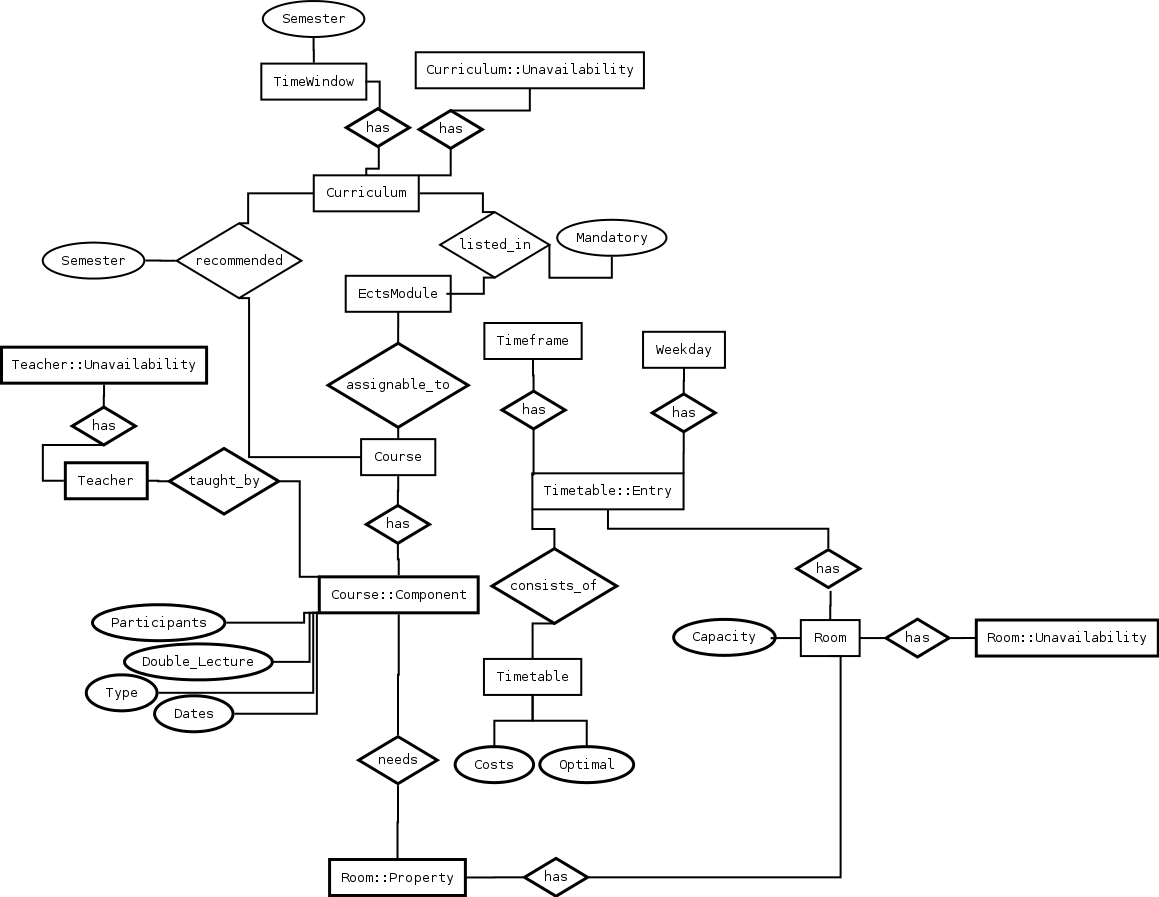
\includegraphics[width=\textwidth]{TimetablingER_Dia.png}
    \caption{Database schema, modeled as entity-relationship diagram \cite{Chen76}.}
    \label{fig:schema}    
\end{figure}

Figure~\ref{fig:schema} demonstrates the database schema.
A timetable, which consists of several timetable entries, represents a complete schedule.
Timetables have costs, resulting from penalty values of the ASP soft constraints.
The timetables with the lowest costs are optimal solutions.
A timetable entry is an assignment of a certain component of a course, e.g. a lecture, to a certain room and a specific weekday and timeframe.
Course components, taught by a specific teacher, have got a certain type, e.g lecture, tutorial, etc.
These components reflect the parts of a course which are to be attended by the student in order to enroll for the course.
As an example, a student needs to attend both lecture and tutorial, but of course he doesn't need to attend \emph{all} the same tutorials which are given by different tutors.
Furthermore, course components can have multiple dates, participants and several room properties.
If, for instance, the course component has to take place in a computer pool then the room assigned to the course component has to be declared as computer pool through a certain property.
Courses belong to a curriculum via an ects module.
Also they can be recommended for a certain semester for a specific curriculum.
During our requirements engineering it turned out that this recommendation has to be independent from the ects module.
The reason here is that courses which belong to the same curriculum via the same module can have a different difficulty.
Secondarily, recommendations are declared by the responsible teacher of the course whereas the commission of the university decides which courses belong to which curricula.
The ects module is then listed in a certain curriculum as compulsory (mandatory) or elective.
Another peculiarity which emerged from the requirements engineering is the existence of time windows.
This is a very special requirement of the university of potsdam.
It ensures that students who become a teacher (``Lehramt'') are able enroll for courses in their multitudinous combination of subjects.
In order to prevent overlapping, mandatory lectures for prospective teachers have to be assigned to a determined set of time windows dependent on the semester recommendation.
Finally there are unavailabilities for teachers, curriculum and rooms.
All unavailabilities are linked to a specific day and time-slot which is not shown in the diagram for clarity reasons.

\subsection{ASP Integration} 

\begin{figure}[h]
    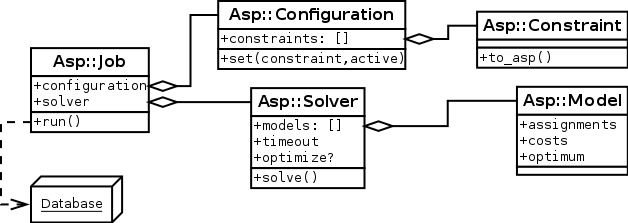
\includegraphics[width=\textwidth]{Images/AspClassDiagram.png}
    \label{fig:class_diagram}
\end{figure}

Figure~\ref{fig:class_diagram} demonstrates the integration of the answer set solving.
In the final encoding we have facts and rules.
A fact corresponds to an entity in the database and a rule corresponds to an \constraint{}.
In order to get all the necessary information from the database to create the desired asp encoding we use the \job{} class.
The main method in this tool chain is the \run{} method.
All entities which are required for the encoding are transformed into facts.
The \job{} then receives a set of constraints from the configuration.
The configuration can enable or disable a certain \constraint{} and in the future it will be used to change the weight of each \constraint{}.
The information is then put together and send to the \solver{} which receives an encoded asp problem as text.
The \solver{} provides the interface to the user's shell and is also responsible to create a \model{} for each found solution.
These \model{} classes are used to parse ruby objects from the strings which are returned by clasp.
So to give an example, every \entry{} is parsed from the answer set.
Also, we parse a violation of a soft constraint from the answer set, associated with the conflicting objects.
Note that violations have to be parsed at the end for this reason.
They are associated to entries of the same answer set which have to be present at the time.
Subsequent to the parsing, the job class then saves all the generated objects in the database.
The state in the database is then used as the input for the visualization of the timetable.

\section{Conclusion}

In summary, we gained very positive experiences within this project using an agile approach to solve the problem.
The planning at the Institute for Computational Science was very complex and there were a large amount of exceptional cases that had to be considered.
Due to our development process we were able to made continuous progress without concentrating too much in the special details.
Besides we had a good relationship to our customer resulting from a mutual exchange of knowledge.
Due to the knowledge transfer we and our customer had a common understanding of the planning problem and we were able to discuss about problems and solution approaches.

%----------------------------------------------------------------------------------------
%	BIBLIOGRAPHY
%----------------------------------------------------------------------------------------
\bibliographystyle{plain}
\bibliography{report}


%----------------------------------------------------------------------------------------

\end{document}
